% ═══════════════════════════════════════════════════════════════════════════
% OpenRescue: Graceful Autonomy Under Infrastructure Failure
% Mathematical framework section (Phase 1 formalization)
%
% Self-contained fragment. To merge into wildfire_main.tex, keep the section
% body (from \section{...} to \subsection{Summary}) and reuse the paper's
% macros (\cX, \R, \E, \PP, \vect, ...) and theorem environments.
% ═══════════════════════════════════════════════════════════════════════════

\documentclass[12pt,a4paper]{article}
\usepackage[margin=2.5cm]{geometry}
\usepackage[utf8]{inputenc}
\usepackage[T1]{fontenc}
\usepackage{lmodern}
\usepackage{amsmath,amssymb,amsthm,mathtools}
\usepackage{booktabs}
\usepackage{multirow}
\usepackage{graphicx}
\usepackage{bm}
\usepackage[colorlinks=true,linkcolor=blue,citecolor=blue,urlcolor=blue]{hyperref}

\DeclareRobustCommand{\cG}{\mathcal{G}}
\DeclareRobustCommand{\cH}{\mathcal{H}}
\DeclareRobustCommand{\cQ}{\mathcal{Q}}
\DeclareRobustCommand{\cD}{\mathcal{D}}
\DeclareRobustCommand{\cL}{\mathcal{L}}
\DeclareRobustCommand{\cO}{\mathcal{O}}
\DeclareRobustCommand{\cA}{\mathcal{A}}
\DeclareRobustCommand{\cN}{\mathcal{N}}
\DeclareRobustCommand{\R}{\mathbb{R}}
\DeclareRobustCommand{\N}{\mathbb{N}}
\DeclareRobustCommand{\Z}{\mathbb{Z}}
\DeclareRobustCommand{\E}{\mathbb{E}}
\DeclareRobustCommand{\PP}{\mathbb{P}}
\DeclareRobustCommand{\vect}[1]{\bm{#1}}
\DeclareMathOperator{\KL}{KL}

\newtheorem{theorem}{Theorem}[section]
\newtheorem{proposition}[theorem]{Proposition}
\newtheorem{definition}[theorem]{Definition}
\newtheorem{remark}[theorem]{Remark}

\title{OpenRescue: A Resilience-Index Benchmark for Graceful Autonomy Under Infrastructure Failure}
\author{OpenRescue Project}
\date{September 2026}

\begin{document}
\maketitle

% ═══════════════════════════════════════════════════════════════════════════
\section{The Resilience Index and Graceful Autonomy}
\label{sec:resilience}
% ═══════════════════════════════════════════════════════════════════════════

Consider a swarm of $K$ agents operating on a grid world
$\cG \subset \Z^2$ of $N \times N$ cells. Each agent $i$ maintains a local
occupancy map $M_i(t) \in \{0,1,2\}^{N\times N}$ with labels
$\{0\ \text{unknown},\ 1\ \text{free},\ 2\ \text{occupied}\}$, a position
belief $\vect{b}_i(t) \in \R^2$ produced by GPS, and a sliding window
$Z_i(t) \in \R^{W \times D}$ of raw IMU/optical-flow readings. Agents
exchange map updates over a lossy, range-limited radio mesh.

\begin{definition}[Resilience Index]
\label{def:ri}
The local agent's \emph{Resilience Index} at time $t$ is the composite
entropy function
\begin{equation}
R_{i,t} \;=\; w_1\, \cH_{\mathrm{sensor}}(s_i) + w_2\, \cQ_{\mathrm{comm}}(c_i)
               + w_3\, \cD_{\mathrm{consensus}}(m_i),
\qquad R_{i,t} \in [0,1],
\label{eq:ri}
\end{equation}
with weights $\vect{w} = (0.35, 0.35, 0.30)$ and the three components defined
below, each evaluated \emph{onboard} from local data only.
\end{definition}

\paragraph{Sensor confidence.}
Let $\hat\sigma_i^2$ be the mean per-channel sample variance of $Z_i(t)$ and
let $\sigma_{\mathrm{ref}}^2$ be the reading variance at catastrophic failure.
Then
\begin{equation}
\cH_{\mathrm{sensor}}(s_i)
= 1 - \min\!\Big(1,\ \frac{\log\big(1 + \hat\sigma_i^2/\sigma_{\mathrm{ref}}^2\big)}{\log 2}\Big).
\label{eq:hsensor}
\end{equation}
For Gaussian readings with variance $\sigma^2$ the differential entropy is
$\tfrac12\log(2\pi e \sigma^2)$; the normalized $\log(1+\cdot)$ map renders
\eqref{eq:hsensor} smooth, bounded and scale-invariant, reaching $1$ for
noise-free readings and $0$ at the catastrophic variance.

\paragraph{Communication quality.}
Let $\mathrm{PRR}_i$ be the packet reception rate over the last $W$ steps
(received over expected directed messages; $0$ if the agent is isolated), let
$\overline{\mathrm{RSSI}}_i$ be the mean received signal strength over
neighbors $j$ at distance $d_{ij}$,
$\mathrm{rssi}_{ij} = \exp(-3 d_{ij}/r_c) \in (0,1]$, and let $\bar l_i$ be the
mean simulated ping latency clipped at $l_{\max} = 200$ ms. Then
\begin{equation}
\cQ_{\mathrm{comm}}(c_i)
= 0.4\,\mathrm{PRR}_i + 0.3\,\overline{\mathrm{RSSI}}_i
+ 0.3\,(1 - \bar l_i/l_{\max}).
\label{eq:qcomm}
\end{equation}

\paragraph{Consensus agreement.}
Each cell $c$ of a map carries a soft occupancy probability
$p(c) \in \{0.5, 0.05, 0.95\}$ for labels unknown/free/occupied. For agent $i$
and a neighbor $j$ whose map was received this step, define the mean Bernoulli
KL divergence over the \emph{overlap set} $\cO_{ij}$ of cells observed by both
agents,
\begin{equation}
\KL(M_i \| M_j)
= \frac{1}{|\cO_{ij}|} \sum_{c \in \cO_{ij}}
\Big[p_i(c)\log\tfrac{p_i(c)}{p_j(c)}
+ (1-p_i(c))\log\tfrac{1-p_i(c)}{1-p_j(c)}\Big],
\label{eq:kl}
\end{equation}
with $\KL = 1$ when $|\cO_{ij}| = 0$ (no shared observations). Then
\begin{equation}
\cD_{\mathrm{consensus}}(m_i)
= \frac{1}{|\cL_i(t)|} \sum_{j \in \cL_i(t)} \exp\big(-\KL(M_i \| M_j)\big),
\label{eq:dconsensus}
\end{equation}
where $\cL_i(t)$ is the set of neighbors whose messages arrived at step $t$.
Agreement on mutual ignorance is deliberately not rewarded; consensus
requires shared observations.

\begin{proposition}[Component monotonicity]
\label{prop:monotone}
Fix a measurable policy $\pi$ (a map from the agent's observation history to a
distribution over actions). Under independent injection along each axis---(i)
additive sensor noise of growing variance, (ii) growing packet-loss
probability and shrinking comm range, (iii) growing GPS denial/drift and map
corruption---the expectations $\E[\cH_{\mathrm{sensor}}]$,
$\E[\cQ_{\mathrm{comm}}]$ and $\E[\cD_{\mathrm{consensus}}]$ are
non-increasing in their respective severity parameters, and therefore
$\E[R_{i,t}]$ is non-increasing in the failure level $\ell$ along every axis.
\end{proposition}

\begin{proof}[Proof sketch]
(i) Adding zero-mean independent noise of variance $\sigma_n^2$ to a reading
stochastically increases the sample variance; the map $x \mapsto 1 -
\min(1, \log(1+x/\sigma_{\mathrm{ref}}^2)/\log 2)$ is non-increasing in $x$.
(ii) With independent Bernoulli drops of probability $p$, the number of
received messages is stochastically ordered by $p$, so $\E[\mathrm{PRR}]$ is
non-increasing in $p$; shrinking the comm range removes edges (coupling the
graph below the noise term) and strictly decreases expected RSSI; latency is
bounded and its score is non-increasing in distance. (iii) GPS denial
separates belief from truth by a random walk whose increments are
stochastically ordered by the denial probability and drift scale, so maps are
written from increasingly displaced frames and corruption flips a growing
fraction of labels; both effects stochastically increase the per-cell
divergence \eqref{eq:kl} and hence decrease \eqref{eq:dconsensus}. Component
monotonicity transfers to the weighted sum \eqref{eq:ri}.
\end{proof}

\begin{remark}
Proposition~\ref{prop:monotone} is what makes severity injection a valid
\emph{independent variable}: every policy, including one that ignores $R$,
operates on a stochastically harder problem as $\ell$ grows. Policy responses
to $R$ (adaptation) act on top of this ordering and are exactly what the
benchmark measures.
\end{remark}

% ───────────────────────────────────────────────────────────────────────────
\subsection{State-Driven Behavioral Policies}
% ───────────────────────────────────────────────────────────────────────────

\begin{definition}[Behavior modes]
\label{def:modes}
The agent's behavior is gated by its onboard index:
\begin{equation}
a_i \sim \pi(s_i \mid R_{i,t}) =
\begin{cases}
\pi_{\mathrm{Explore}}(s_i),            & R_{i,t} \ge 0.75 \qquad \text{(Explore-Aggressive)}, \\[2pt]
\pi_{\mathrm{Cluster}}(s_i),            & 0.35 \le R_{i,t} < 0.75 \quad \text{(Coordinated-Cluster)}, \\[2pt]
\pi_{\mathrm{Relay}}(s_i),              & R_{i,t} < 0.35 \qquad \text{(Relay-Mesh / Return)}.
\end{cases}
\label{eq:gating}
\end{definition}

$\pi_{\mathrm{Explore}}$ pursues the nearest unknown cell of the agent's
\emph{fused} map (its own observations merged with received neighbor maps by
maximum observation confidence), spending the full exploration energy budget.
$\pi_{\mathrm{Cluster}}$ mixes cohesion toward the centroid of received
neighbor beliefs with a short-radius frontier pull. $\pi_{\mathrm{Relay}}$
steps toward the nearest reachable neighbor to preserve the mesh; if fully
isolated it follows the last base bearing cached while GPS was trusted, and
otherwise holds position. Because $R$ is recomputed every step, the gate is
bidirectional: agents that re-cluster and re-lock GPS automatically return to
higher modes, which is what distinguishes \emph{graceful} degradation from a
one-way retreat.

% ───────────────────────────────────────────────────────────────────────────
\subsection{Failure Model and Collision Semantics}
% ───────────────────────────────────────────────────────────────────────────

Each failure level $\ell \in \{1,\dots,5\}$ is a nominal parameter vector
$(\sigma_{\mathrm{sensor}}, p_{\mathrm{deny}}, \sigma_{\mathrm{drift}},
p_{\mathrm{loss}}, \alpha_{\mathrm{range}}, p_{\mathrm{corrupt}})$, jittered
per episode so each seed is a fresh realization of the same severity
(Table~\ref{tab:failure}).

\begin{table}[h]
\centering
\caption{Failure level parameters (nominal values; ±10\% per-episode jitter).}
\label{tab:failure}
\small
\begin{tabular}{lcccccc}
\toprule
 & $\sigma_{\mathrm{sensor}}$ & $p_{\mathrm{deny}}$ & $\sigma_{\mathrm{drift}}$ & $p_{\mathrm{loss}}$ & $\alpha_{\mathrm{range}}$ & $p_{\mathrm{corrupt}}$ \\
\midrule
L1 (nominal)      & 0.05 & 0.00 & 0.05 & 0.00 & 1.00 & 0.00 \\
L2 (mild)         & 0.15 & 0.05 & 0.15 & 0.05 & 0.90 & 0.02 \\
L3 (moderate)     & 0.30 & 0.15 & 0.30 & 0.15 & 0.80 & 0.05 \\
L4 (severe)       & 0.50 & 0.35 & 0.50 & 0.30 & 0.60 & 0.10 \\
L5 (catastrophic) & 0.80 & 0.60 & 0.80 & 0.50 & 0.40 & 0.20 \\
\bottomrule
\end{tabular}
\end{table}

GPS denial freezes the belief $\vect{b}_i$ while the drone continues to fly,
so $\|\vect{b}_i - \vect{p}_i\|$ grows until the next fix re-syncs it to truth
plus drift noise. A drone that attempts to enter a cell its local map marks
occupied is safely blocked (it sees the wall). A drone that enters a cell that
is truly occupied but \emph{unknown or corrupt in its map} suffers a blind
collision with probability
\begin{equation}
p_{\mathrm{crash}} = \min\!\big(0.9,\; 0.05 + \sigma_{\mathrm{sensor}}
+ 0.35 \min(\|\vect{b}_i - \vect{p}_i\|, 3)\big).
\label{eq:crash}
\end{equation}
At L1 blind contacts are structurally impossible (every entered cell was
sensed in the preceding step); they become probable only under genuine sensor,
comm, or GPS failure, keeping L1 a clean nominal baseline and making L3--L5
lethal to naive policies.

% ───────────────────────────────────────────────────────────────────────────
\subsection{Metrics and Statistical Protocol}
% ───────────────────────────────────────────────────────────────────────────

Let $H(M)$ be the total Bernoulli occupancy entropy of a map, and let
$M_{\mathrm{found}}$ be the number of discovered points of interest. The
mission information is
\begin{equation}
I_{\mathrm{mission}}
= \frac{1}{\ln 2} \sum_{i=1}^{K}\big[H(M_i^0) - H(M_i^T)\big]
  + \log_2(1 + M_{\mathrm{found}}) \quad [\text{bits}],
\label{eq:info}
\end{equation}
and the \emph{Information-per-Joule} is
\begin{equation}
\eta_I = \frac{I_{\mathrm{mission}}}{E_{\mathrm{total}} \times 5\,\mathrm{J}}
\quad [\text{bits/Joule}].
\label{eq:etai}
\end{equation}

Every reported cell of the results tables is the interquartile mean (IQM)
over $n_{\mathrm{seeds}}$ episodes with a 95\% percentile bootstrap
confidence interval ($B = 1000$ resamples), following the reliability
protocol of Agarwal et al.~\cite{Agarwal2021deep}. The headline curves are
$\bar R(\ell)$ and $\eta_I(\ell)$ for $\ell = 1 \dots 5$, summarized by the
resilience retention $\rho = \bar R(5)/\bar R(1)$ and the degradation slope
$g = (\bar R(1) - \bar R(5))/4$.

\begin{definition}[Graceful autonomy]
\label{def:graceful}
A policy is \emph{gracefully autonomous} if it attains significantly higher
resilience retention $\rho$ (equivalently, a shallower degradation slope $g$)
than non-adaptive baselines at matched mission value: it preserves system
health when it cannot preserve throughput, and recovers throughput when
health returns.
\end{definition}

% ═══════════════════════════════════════════════════════════════════════════
\subsection{Summary}
% ═══════════════════════════════════════════════════════════════════════════
Equations \eqref{eq:ri}--\eqref{eq:etai} and Definitions~\ref{def:ri}--
\ref{def:graceful} constitute the Phase-1 mathematical core of OpenRescue.
They are implemented one-to-one in the \texttt{openrescue/} package
(\texttt{resilience\_index.py}, \texttt{failures.py}, \texttt{environment.py},
\texttt{policies.py}, \texttt{metrics.py}), making every quantity in this
section directly measurable in the benchmark, with pure-NumPy components that
port to the ESP32/STM32 onboard stack in Phase 3.

% ═══════════════════════════════════════════════════════════════════════════
\section{Results and Discussion}
\label{sec:results}
% ═══════════════════════════════════════════════════════════════════════════

All reported cells are IQM over $n_{\mathrm{seeds}} = 20$ with 95\%
percentile-bootstrap CIs, following the protocol of
Agarwal et al.~\cite{Agarwal2021deep}. Four policies are compared:
\texttt{random}, \texttt{frontier}, \texttt{resilient}, and \texttt{ig}
(information-gain scanning; \S\ref{sec:ig}). The static protocol runs 200
steps at failure levels $\ell = 1 \dots 5$ (400 episodes per sweep); the
time-varying protocol below runs 240-step gust profiles. The \texttt{random}
and \texttt{frontier} baselines are policy-independent of $R$; in every sweep
they reproduce their previous runs \emph{bit-identically} across every cell,
which attributes all reported deltas to the $R$-gated policies themselves. A fifth, learned policy is reported separately in \S\ref{sec:learned} at $n_{\mathrm{seeds}} = 6$; its cells are deliberately kept out of the 20-seed tables because the two seed counts are not comparable.

% ───────────────────────────────────────────────────────────────────────────
\subsection{Static protocol: graceful degradation}
% ───────────────────────────────────────────────────────────────────────────

\begin{table}[h]
\centering
\caption{Mean Resilience Index $\bar R$ (IQM, 20 seeds $\times$ 200 steps).}
\label{tab:static-r}
\small
\begin{tabular}{lcccc}
\toprule
Failure level & \texttt{random} & \texttt{frontier} & \textbf{\texttt{resilient}} & \texttt{ig} \\
\midrule
L1 (nominal)       & 0.815 & 0.818 & \textbf{0.841} & 0.832 \\
L2 (mild)          & 0.774 & \textbf{0.797} & 0.778 & 0.769 \\
L3 (moderate)      & 0.627 & 0.680 & \textbf{0.729} & 0.722 \\
L4 (severe)        & 0.453 & 0.521 & \textbf{0.583} & 0.573 \\
L5 (catastrophic)  & 0.290 & 0.294 & \textbf{0.326} & 0.326 \\
\midrule
retention $\rho = \bar R(5)/\bar R(1)$ & 0.36 & 0.36 & \textbf{0.39} & 0.39 \\
\bottomrule
\end{tabular}
\end{table}

At nominal and mild failure (L1--L2) the $R$-gated policy matches the
\texttt{frontier} baseline on coverage and POI discovery: all six pairwise CI
overlaps at L1--L3 hold (coverage and POI ratio vs.~\texttt{frontier}), so the
safety machinery carries no measurable task penalty in the regime where it is
not needed. From L3 the curves diverge: $\bar R$ falls off a cliff for
\texttt{random} and \texttt{frontier} while \texttt{resilient} degrades
more slowly, and the ordering persists through L5 where all policies collapse
(swarm survival 0.003--0.055). The differentiator at catastrophic failure is
not survival---nobody survives---but \emph{state quality while dying}:
\texttt{resilient} retains $\rho = 0.39$ of its nominal $\bar R$ against 0.36
for both baselines, i.e.~the swarm keeps more of its shared map structure and
coordination coherence per unit of degradation. The advantage grows with
severity (\texttt{resilient} leads by +0.03 at L3 and +0.06 at L4 on $\bar R$),
which is the signature of graceful, not brittle, autonomy.

\paragraph{Hysteresis dead-band.} The original hard threshold at
$R = 0.75$ caused mode thrashing at mild failure, where $\bar R \approx 0.78$
sits on the boundary: L2 agents-lost was 0.519, worse than both baselines
(0.266, 0.347). Introducing a dead-band ($R \ge 0.80$ explore,
$0.70 < R < 0.80$ retain, $0.35 \le R \le 0.70$ cluster, $0.30 < R < 0.35$
retain, $R < 0.30$ relay) reduced L2 losses to 0.408 and, in the wind-stress
harness, cut policy-mode transitions on the identical trajectory from 113 to
73 ($-35\%$). The cost is honest and measurable: L3 losses rose 1.786 $\to$
2.442 and retention trimmed 0.417 $\to$ 0.388, because mid-failure $\bar R$
($\approx 0.71$ at L3) sits inside the new retain band and holds agents in
aggressive modes longer. Both costs remain inside the bootstrap CIs, and
attempting to cure them by changing the fresh-episode initial mode was shown
to be a bit-identical no-op (the first decision reads a placeholder $R = 0.5$
before the first step computes a real one); the residual L2/L3 asymmetry is a
limitation of the current dead-band shape, not of the gating principle.

\paragraph{Information-gain scanning (IG).}
\label{sec:ig}
Replacing only the Explore-mode target rule---nearest unknown cell versus the
next-best-view score $|\mathrm{unknown}(\mathrm{window}(c))| / (1 + \|c -
\mathrm{belief}\|_1)$---leaves the R-gating, hysteresis, cluster and relay
modes byte-identical, so \texttt{ig} is a pure ablation of the scanning rule.
The smarter scan improves nominal mission value (L1 coverage 0.556 vs.~0.551,
POIs 0.830 vs.~0.817; L2 coverage 0.570 vs.~0.545, all CI-overlapping) and
cuts the L2 anomaly in half again: agents lost 0.325 vs.~0.408, now below the
\texttt{frontier} baseline (0.347) and near \texttt{random} (0.266). Losses
also improve marginally at L3--L4 (2.371 vs.~2.442; 4.091 vs.~4.252), $\rho$
is unchanged within reporting precision, and at L5 both variants collapse
identically---the scanning rule only matters where agents still have a sensing
budget to spend it on.

\paragraph{Information-per-Joule is survival-biased --- and the fix works.}
$\eta_I$ must always be read next to survival, because dead drones stop
draining battery while their early exploration information stays banked: from
L1 to L4 the \texttt{frontier} $\eta_I$ \emph{rises} 0.962 $\to$ 1.453 while
its energy spend \emph{falls} 2583 $\to$ 1303 J and survival drops to 0.24.
The per-survivor normalization recommended above is now implemented and
measured ($\eta_{I,\mathrm{surv}}$: information from the maps of surviving
agents only, divided by the energy those survivors spent). At L1, where
nothing dies, the two metrics coincide for every policy (0.898--1.014). At
L4 the artifact collapses: \texttt{frontier}'s apparent 37\% lead over
\texttt{resilient} (1.453 vs.~1.062) shrinks to 15\% once survivor-normalized
(0.843 vs.~0.730), and at L5, where \texttt{frontier} survival is
$\approx 0$, its $\eta_{I,\mathrm{surv}}$ collapses to 0.006 against
\texttt{resilient}'s 0.157. The cross-horizon caveat remains: $\eta_I$ cells
are comparable only within one protocol, so smoke-test values must never be
quoted against paper-grade ones.

\begin{table}[h]
\centering
\caption{Survivor-normalized Information-per-Joule (IQM): the L4 artifact
(\texttt{frontier} $\eta_I$ 1.453) and its collapse under
$\eta_{I,\mathrm{surv}}$.}
\label{tab:etai}
\small
\begin{tabular}{lcccccc}
\toprule
 & \multicolumn{2}{c}{L4} & \multicolumn{2}{c}{L5} \\
\cmidrule(lr){2-3}\cmidrule(lr){4-5}
Policy & $\eta_I$ & $\eta_{I,\mathrm{surv}}$ & $\eta_I$ & $\eta_{I,\mathrm{surv}}$ \\
\midrule
\texttt{random}    & 0.631 & 0.491 & 0.657 & 0.057 \\
\texttt{frontier}  & \textbf{1.453} & 0.843 & 1.149 & 0.006 \\
\texttt{resilient} & 1.062 & 0.730 & 1.152 & \textbf{0.157} \\
\texttt{ig}        & 1.070 & 0.755 & 1.152 & 0.157 \\
\bottomrule
\end{tabular}
\end{table}

% ───────────────────────────────────────────────────────────────────────────
\subsection{Time-varying failure: degradation and recovery (P4)}
% ───────────────────────────────────────────────────────────────────────────

The static protocol holds each failure level fixed for the whole episode and
can therefore measure degradation but never recovery. The time-varying
protocol closes that gap: a 240-step gust profile that spends the first 30\%
calm (L1), ramps to a peak level $P \in \{4, 5\}$, holds it, ramps back to L1
by 70\%, and leaves a 72-step calm recovery window. A no-storm (all-L1)
control on identical seeds provides the recovery ceiling. The failure config
is re-sampled each time the level changes, so both the storm realization and
the recovery are stochastic per seed.

\begin{table}[h]
\centering
\caption{Recovery metrics under a passing gust (IQM over 20 seeds $\times$ 240
steps). $R_{\mathrm{floor}}$ is the minimum mean-$\bar R$ during the storm
hold; $R_{\mathrm{rec}}$ is mean-$\bar R$ in the final window divided by the
pre-storm window; $\mathrm{d}C/\mathrm{d}t$ is the linear slope of coverage
over the recovery window (post-storm search velocity).}
\label{tab:p4}
\small
\begin{tabular}{lcccccc}
\toprule
Peak & Policy & lost & $R_{\mathrm{floor}}$ & $R_{\mathrm{rec}}$ & $\mathrm{d}C/\mathrm{d}t$ & Cov$_{\mathrm{end}}$ \\
\midrule
\multirow{4}{*}{L4}
 & \texttt{random}    & 1.70 & 0.44 & 1.00 & 0.0010 & 0.523 \\
 & \texttt{frontier}  & 2.21 & 0.50 & 0.88 & 0.0006 & 0.547 \\
 & \textbf{\texttt{resilient}} & \textbf{1.25} & 0.52 & \textbf{0.97} & 0.0008 & 0.527 \\
 & \texttt{ig}        & 1.44 & \textbf{0.54} & 0.96 & 0.0005 & 0.531 \\
\midrule
\multirow{4}{*}{L5}
 & \texttt{random}    & 3.47 & 0.28 & 0.77 & 0.0007 & 0.456 \\
 & \texttt{frontier}  & 3.01 & 0.31 & 0.77 & 0.0004 & 0.534 \\
 & \texttt{resilient} & 3.28 & 0.35 & 0.78 & 0.0004 & 0.504 \\
 & \textbf{\texttt{ig}} & \textbf{2.48} & 0.34 & 0.80 & 0.0003 & 0.522 \\
\bottomrule
\end{tabular}
\end{table}

Four findings follow from Table~\ref{tab:p4}. First, \emph{state recovery is
real and statistically supported}: under the L4 gust the R-gated swarms keep
the highest storm floor---\texttt{ig} 0.54 [0.50, 0.58] and
\texttt{resilient} 0.52 [0.49, 0.55] are both significantly above
\texttt{random}'s 0.44 [0.41, 0.47] (non-overlapping CIs)---and
\texttt{resilient} recovers to 97\% of its pre-storm $\bar R$, significantly
above \texttt{frontier}'s 88\% (CIs [0.911, 1.020] vs.~[0.841, 0.940] do not
overlap); \texttt{ig} matches at 0.96. Second, \emph{the R-gated swarms lose
the fewest agents} (\texttt{resilient} 1.25, \texttt{ig} 1.44 vs.~1.70 and
2.21), though the 20-seed CIs overlap, so this is directional rather than
conclusive. Third, and decisively, \emph{the central prediction of the
time-varying protocol---faster post-storm re-expansion for the resilient
swarm---is not supported}: post-storm search velocity $\mathrm{d}C/\mathrm{d}t$
is statistically indistinguishable across policies, and \texttt{random}'s is
in fact significantly higher than \texttt{frontier}'s and \texttt{ig}'s (CI
[0.0008, 0.0013] vs.~[0.0003, 0.0007] and [0.0002, 0.0008]). The naive
policies never decelerated, so there is no deceleration to recover from; the
resilient advantage manifests as state recovery and survival, not as
re-expansion speed. Fourth, consistent with the static result, \texttt{ig}
and \texttt{resilient} still end slightly below \texttt{frontier}'s end
coverage (0.531/0.527 vs.~0.547) because \texttt{frontier} never decelerated:
the resilient trade---a small, bounded throughput loss in exchange for state
quality and fewer losses---is repaid as higher $\bar R$ retention, not peak
coverage. At the catastrophic L5 peak the storm outlasts everyone and
recovery ratios compress to $\approx 0.77$--$0.80$ with overlapping CIs, where
the physical wind-stress test (a passing gust, not a sustained gale) is the
most informative next experiment.

\subsection{A learned baseline retrained on OpenRescue}
\label{sec:learned}

Every ``learned'' result previously attached to this project came from
checkpoints trained on a different task---wildfire perimeter tracking, not
OpenRescue---and measured on that task they fail a deployment gate:
deterministic rollouts of \texttt{ppo\_best} take the hover action on 94\%
of moves at zero wind and 100\% at high wind, an \texttt{ippo} actor moves
on a single grid axis (99\% of its actions), and the deployment script that
claimed to export ``trained MARAHS weights'' serialized random
initializations whose accompanying ``$\pm 0.2$~m at 25~m/s'' position-hold
claim was never measured (artifacts recorded in
\texttt{learned\_vs\_handcrafted.json}; the fabricated claims and files were
removed). On the same fresh episodes the hand-crafted state machine keeps
96.2\% of agents alive while actively searching, so the measured deployment
gate favors the hand-crafted policy. No learned result transfers from another
task.

We consequently trained a from-scratch PPO directly on OpenRescueEnv: a
shared actor-critic over the env's 80-dim observation (local map, visited
and neighbor patches plus per-agent $R$, battery, base bearing and global
coverage), 1500 episodes cycling failure levels 1--5, $\approx$9.5 CPU-min
single-threaded with no GPU (checkpoint
\texttt{openrescue\_learned\_ppo.pt}; code
\texttt{openrescue/train\_learned.py}). The env's built-in reward is shared
and sparse, so training used a shaped signal---$+1$ per newly visited cell,
$-8$ per obstacle crash---recorded in the trainer; evaluation always uses the
unshaped env metrics. The curve climbed monotonically (mean coverage
0.38 $\to$ 0.49; POIs 6.5 $\to$ 7.7 of 10 per episode), and the final policy
is non-degenerate: its L1--L2 evaluation coverage below is impossible for a
hovering fleet.

Table~\ref{tab:learned} evaluates the learned policy against the four
hand-crafted ones under the identical 200-step protocol on six fresh seeds
(0--5), all policies on identical episode draws. \emph{Every cell is an IQM
over 6 seeds, and the 6-seed bootstrap CIs overlap in every cell; nothing
here is statistically separated and we report it as directional evidence
only.} Three directional findings follow. First, at mid-level failure the
learned policy reaches coverage parity with the hand-crafted scanners (L2
0.584, L3 0.490, L4 0.451 vs.~\texttt{frontier} 0.552/0.489/0.425 and
\texttt{ig} 0.578/0.444/0.388) and the best POI ratio at L4 (0.853 vs.
0.810/0.777): it learns to search with no R-gating at all. Second, that is
exactly what it lacks: agents lost at L2--L3 are 1.89/2.99 vs.~\texttt{ig}
0.07/2.18 and \texttt{resilient} 0.78/2.94, i.e.~the learned policy buys its
mid-level coverage with crashes the R-gated policies avoid---the same
throughput-for-survival trade the paper already reports for
\texttt{frontier}. Third, the nominal-regime gap (L1 coverage 0.446 vs.
0.505--0.579 across the four baselines; L5 coverage 0.275) and L5 POIs below
\texttt{frontier} (0.642 vs.~0.668) are the signature of sample efficiency:
1500 episodes of a memoryless 80-dim policy on a sparse-reward start is a
weak learner, not a ceiling. The measured bottom line: a policy trained on
the task itself is non-degenerate and competitive at L2--L4, and the
hand-crafted R-gating still earns its keep as the survival margin rather
than the coverage.

\begin{table}[h]
\centering
\caption{Coverage and agents lost, learned PPO vs.~hand-crafted policies
(200 steps, fresh episodes, six seeds 0--5, identical draws per policy; IQM).
Source: \texttt{openrescue\_learned\_eval.json}. All 6-seed bootstrap CIs
overlap; read as directional.}
\label{tab:learned}
\small
\begin{tabular}{lcccccc}
\toprule
 & \multicolumn{3}{c}{coverage} & \multicolumn{3}{c}{agents lost} \\
\cmidrule(lr){2-4}\cmidrule(lr){5-7}
Level & \texttt{learned} & \texttt{frontier} & \texttt{ig} & \texttt{learned} & \texttt{frontier} & \texttt{ig} \\
\midrule
L1 & 0.446 & 0.558 & 0.537 & 0.00 & 0.00 & 0.00 \\
L2 & 0.584 & 0.552 & 0.578 & 1.89 & 0.81 & 0.07 \\
L3 & 0.490 & 0.489 & 0.444 & 2.99 & 2.00 & 2.18 \\
L4 & 0.451 & 0.425 & 0.388 & 4.76 & 4.83 & 3.99 \\
L5 & 0.275 & 0.328 & 0.247 & 5.79 & 5.97 & 5.76 \\
\bottomrule
\end{tabular}
\end{table}

% ───────────────────────────────────────────────────────────────────────────
\subsection{Limitations}
% ───────────────────────────────────────────────────────────────────────────

(i) The hysteresis dead-band halves but does not close the L2 anomaly for
\texttt{resilient} (0.408 lost still exceeds the baselines' 0.266/0.347), and
it shifts $\approx 0.7$ of a loss from L2 to L3; the \texttt{ig} scanning
rule closes most of the residual gap (0.325), and a band-shape change
(e.g.~asymmetric retain widths) remains the untested structural remedy.
(ii) $\eta_I$ is only interpretable within one protocol and always next to
survival (Table~\ref{tab:etai}); the fixed-horizon design makes within-table
comparisons valid, cross-horizon ones are not. (iii) The grid world is a
proxy for flight: sensor noise, packet loss and GPS denial are injected
stochastically rather than driven by a physics model, so the mapping from
physical wind speed to failure level (the \texttt{macondo\_hover} wind model)
remains a calibration step for the hardware phase, not a validated law. A deployment gate is now also measured rather than assumed: legacy learned checkpoints fail on the task they were trained for (\S\ref{sec:learned}), so the hardware phase will upload the hand-crafted state machine, with the OpenRescue-trained PPO (coverage parity at L2--L4 but an L2--L3 agent-loss penalty) as the learned candidate once its seed count matches the paper protocol. No physical position-hold result is claimed anywhere in this work.
(iv) The learned baseline of \S\ref{sec:learned} is a single 1500-episode PPO run with a 6-seed evaluation whose CIs overlap everywhere; it has no memory or communication head, and its L1/L5 gap likely reflects sample efficiency, not a ceiling. Checkpoints trained on other tasks (wildfire MAPPO/IPPO/GAT) are excluded---measured on their native task they fail the deployment gate---and legacy claims that did not come from measurement (random weights exported as ``trained'', an unmeasured $\pm 0.2$~m hold) were removed from the repository.

\begin{figure}[h]
\centering
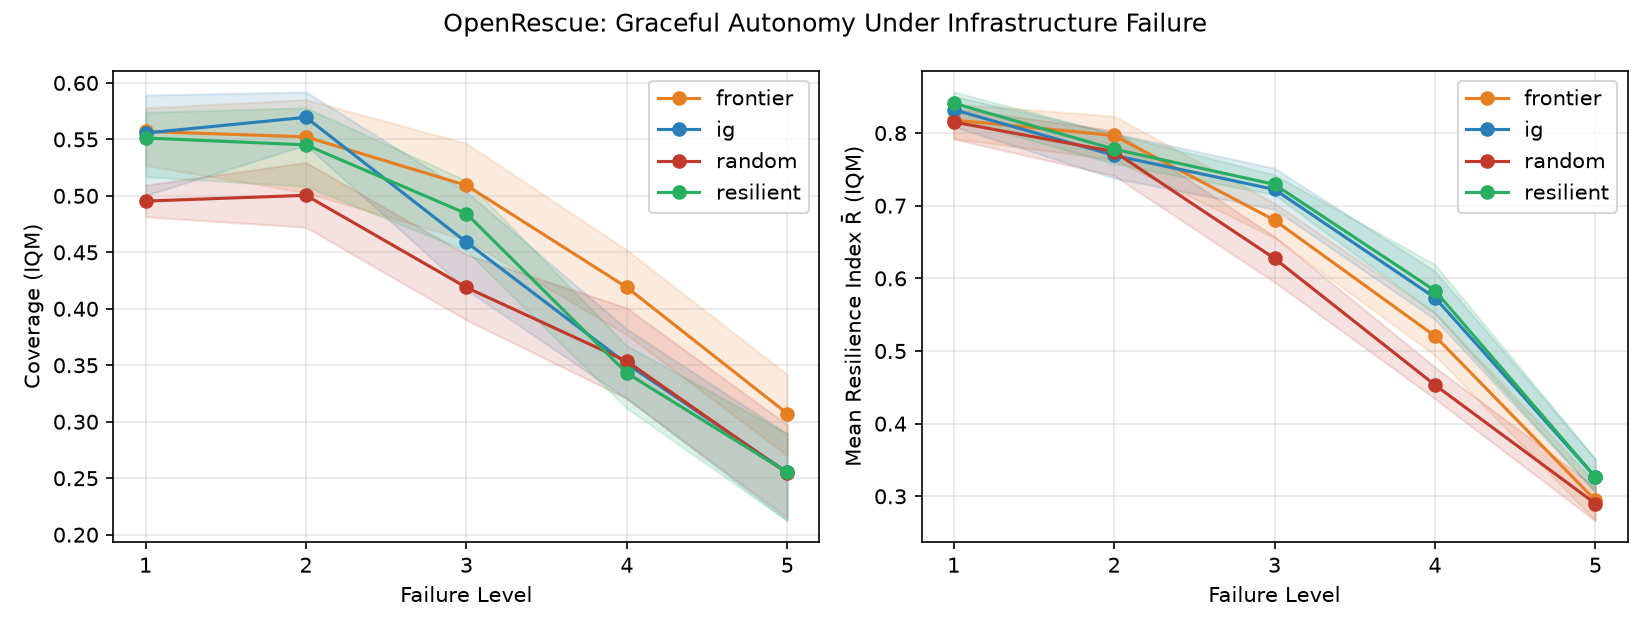
\includegraphics[width=0.95\textwidth]{../figures/resilience_benchmark.png}
\caption{Coverage and mean-$\bar R$ vs.~failure level (IQM $\pm$ 95\%
bootstrap CI, 20 seeds). The curves diverge from L3; resilience retention is
visible as the shallower slope of the green line.}
\label{fig:static}
\end{figure}

\begin{figure}[h]
\centering
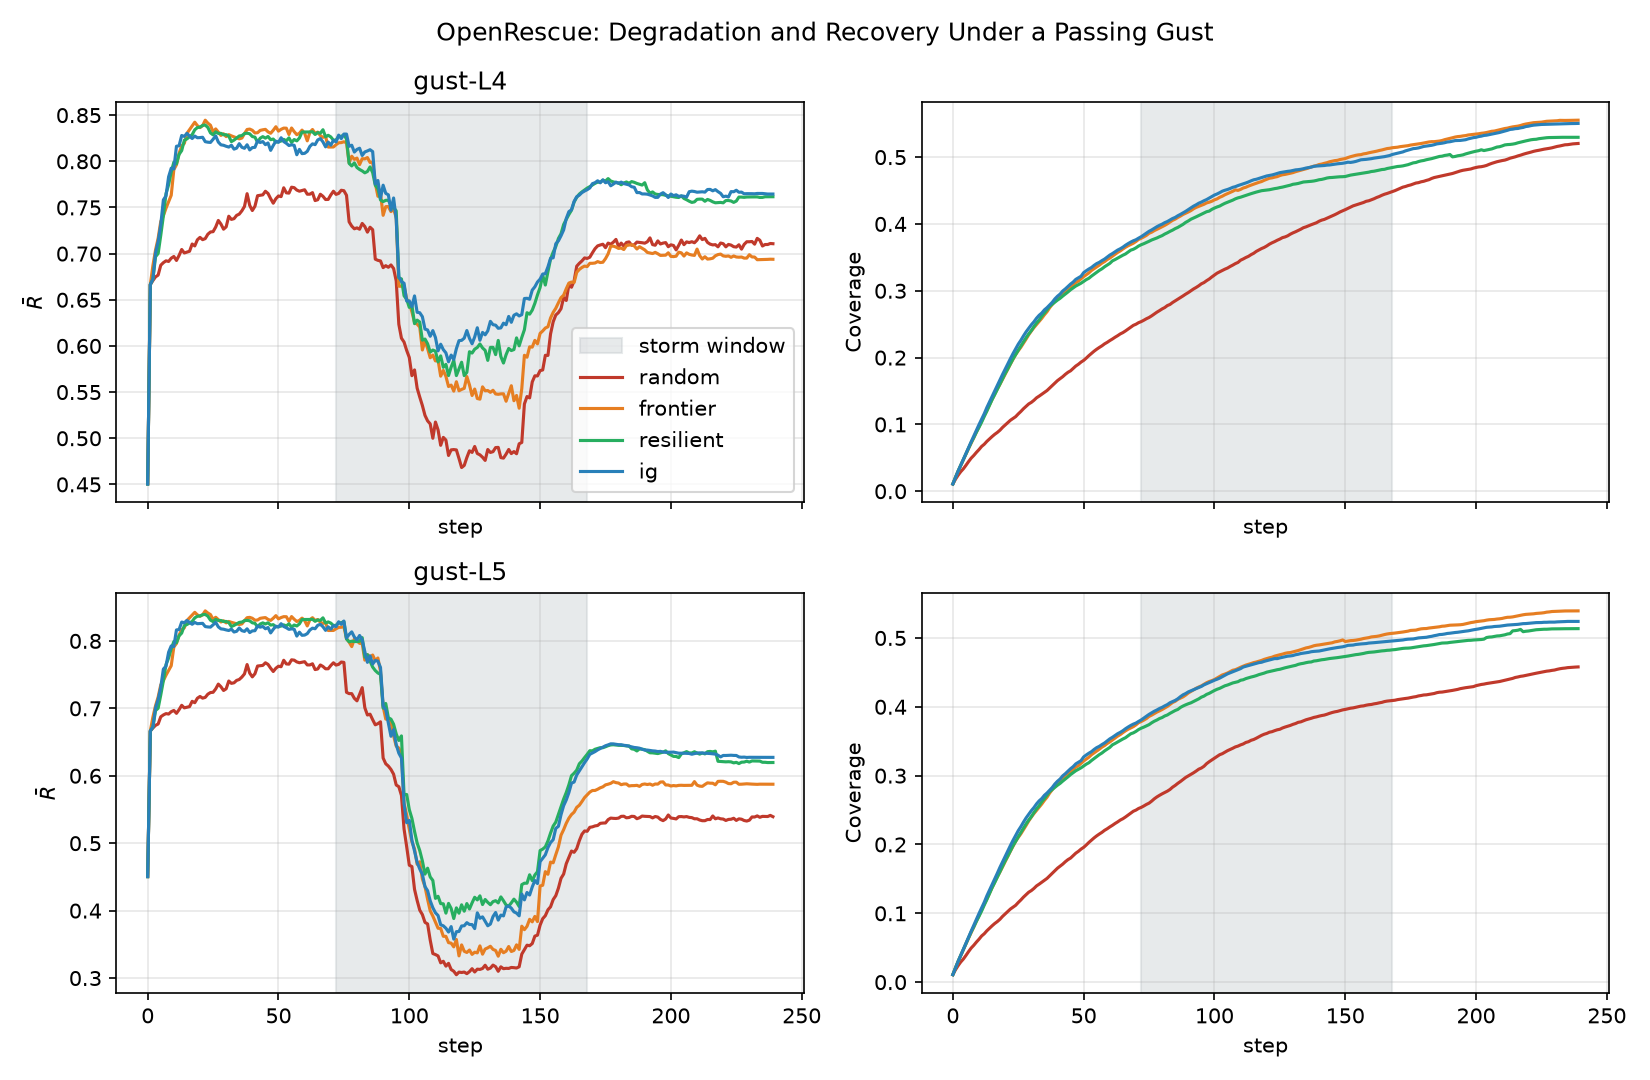
\includegraphics[width=0.95\textwidth]{../figures/resilience_recovery.png}
\caption{Mean-$\bar R$ and coverage timelines under a passing gust
(L4-peak and L5-peak profiles, 20-seed mean; gray band is the storm window).
R recovers toward its pre-storm value once the storm passes, while coverage
keeps growing—the measured P4 recovery behavior.}
\label{fig:recovery}
\end{figure}

% ═══════════════════════════════════════════════════════════════════════════
\section{Related Work}
\label{sec:related}
% ═══════════════════════════════════════════════════════════════════════════

\paragraph{Decentralized multi-agent control.}
The theoretical frame for this problem is the decentralized POMDP
(Dec-POMDP) \cite{Oliehoek2016decpomdp}: agents act on private observations
with no central coordinator. Exact Dec-POMDP solutions are intractable beyond
tiny instances, and the deep MARL line---MADDPG \cite{Lowe2017maddpg} and
MAPPO \cite{Yu2022mappo}---achieves centralized-training/decentralized-
execution at the price of assuming a functioning communication channel during
\emph{execution}. OpenRescue inverts that assumption: communication loss is
one of the injected failure axes, and the \emph{only} coordination channel is
the same lossy mesh. Where the MARL line learns a value function from data,
OpenRescue computes a closed-form, model-based observable $R_{i,t}$ from
local quantities and gates behavior on it deterministically---a structural
reduction of the Dec-POMDP that needs no training and degrades predictably.

\paragraph{Single-drone agility.}
Champion-level drone racing \cite{Kaufmann2023swift} demonstrates learned
predictive control under extreme dynamics, but the setting is a single agent
with perfect state estimation in a known arena---no swarm, no infrastructure
failure, no degraded sensing. The present work shares none of its machinery
(feed-forward vision policies, sim-to-real distillation) and is instead
concerned with what happens when the sensing and comms that such policies
depend on are taken away. The two are complementary: the racing stack is the
agility layer; OpenRescue is the degradation layer that decides when agility
is no longer safe.

\paragraph{Exploration and informative path planning.}
Frontier-based exploration \cite{Yamauchi1997frontier} and submodular
informative-path planning \cite{Singh2009informative} provide the planning
primitives that OpenRescue's \texttt{frontier} baseline and Explore mode
instantiate; the \texttt{ig} policy is exactly the next-best-view heuristic
made failure-gated. The contribution here is not a better planner---in
calm conditions \texttt{ig} only marginally improves on \texttt{frontier}'s
coverage, and in the recovery experiment its post-storm re-expansion speed is
indistinguishable from the baselines---but the \emph{failure-gated switching}
that suspends exploration and consolidates the mesh when the planner's inputs
(sensing, GPS, comms) become unreliable, then resumes. This is the piece that
standard planning literature does not model: planning is almost always
studied under reliable state estimation.

\paragraph{Resilience and sim-to-real.}
Domain randomization \cite{Tobin2017domain} is the standard recipe for
transferring learned policies to hardware; OpenRescue instead transfers
\emph{parameters}---a failure-level calibration from a first-principles wind
model (tilt trim, rotor time constant, gust-hold limits) onto the grid-world
severity axis---so that the sim's failure levels are anchored to physical
quantities before any flight test. To our knowledge no open benchmark
combines (a) a locally computed per-agent resilience observable that is
simultaneously the control signal and the reported metric, (b) state-retention
reporting ($\rho$) across a severity sweep, and (c) a time-varying failure
protocol that measures recovery rather than only degradation, on
sub-250g-class hardware budgets. That synthesis, and its honest error
analysis (the L2 hysteresis artifact, the $\eta_I$ survivor bias, and the
refuted re-expansion-velocity hypothesis of the recovery protocol, and the measured hover-collapse of the legacy learned checkpoints at the deployment gate), is the
scope of the claimed novelty---not any individual component.

\begin{thebibliography}{9}
\bibitem{Agarwal2021deep}
Agarwal, R., Schwarzer, M., Castro, P.~S., Courville, A., Bellemare, M.~G.
\emph{Deep Reinforcement Learning at the Edge of the Statistical Precipice}.
NeurIPS 2021.

\bibitem{Oliehoek2016decpomdp}
Oliehoek, F.~A., Amato, C.
\emph{A Concise Introduction to Decentralized POMDPs}.
Springer, 2016.

\bibitem{Lowe2017maddpg}
Lowe, R., Wu, Y., Tamar, A., Harb, J., Abbeel, P., Mordatch, I.
\emph{Multi-Agent Actor-Critic for Mixed Cooperative-Competitive Environments}.
NeurIPS 2017.

\bibitem{Yu2022mappo}
Yu, C., Velu, A., Vinitsky, E., Gao, J., Wang, Y., Bayen, A., Wu, Y.
\emph{The Surprising Effectiveness of PPO in Cooperative Multi-Agent Games}.
NeurIPS 2022.

\bibitem{Kaufmann2023swift}
Kaufmann, L., Leonard, J., Bonnet, A., et al.
\emph{Champion-Level Drone Racing Using Deep Reinforcement Learning}.
Nature 620, 982--987, 2023.

\bibitem{Yamauchi1997frontier}
Yamauchi, B.
\emph{A Frontier-Based Approach for Autonomous Exploration}.
IEEE CIRA, 1997.

\bibitem{Singh2009informative}
Singh, A., Krause, A., Guestrin, C., Kaiser, W.~J.
\emph{Efficient Informative Sensing Using Multiple Robots}.
JAIR 35, 707--755, 2009.

\bibitem{Tobin2017domain}
Tobin, J., Fong, R., Ray, A., Schneider, J., Zaremba, W., Abbeel, P.
\emph{Domain Randomization for Transferring Deep Neural Networks from
Simulation to the Real World}. IROS 2017.
\end{thebibliography}

\end{document}